\begin{figure}[t]
    \vspace*{-\figskipabove px}
    \vspace*{4px}
    \centering
    \begin{subfigure}[t]{0.235\textwidth}
        \vspace{0px}\centering
        % 306
        \begin{subfigure}[t]{0.48\textwidth}
            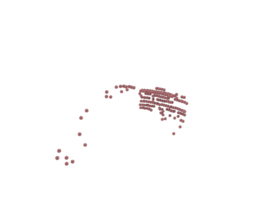
\includegraphics[width=1.75cm,trim={\cropleft cm \croplower cm \cropright cm \cropupper cm},clip]{gdat_kitti_1530_points}
        \end{subfigure}
        \begin{subfigure}[t]{0.48\textwidth}
            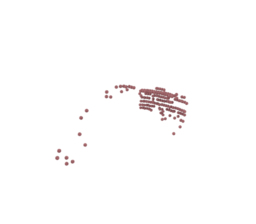
\includegraphics[width=1.75cm,trim={\cropleft cm \croplower cm \cropright cm \cropupper cm},clip]{gdat_kitti_1530_gt}
        \end{subfigure}
        \\
        \begin{subfigure}[t]{0.48\textwidth}
            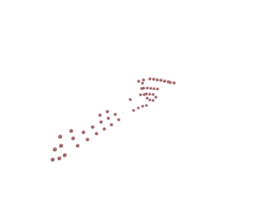
\includegraphics[width=1.75cm,trim={\cropleft cm \croplower cm \cropright cm \cropupper cm},clip]{gdat_kitti_2448_points}
        \end{subfigure}
        \begin{subfigure}[t]{0.48\textwidth}
            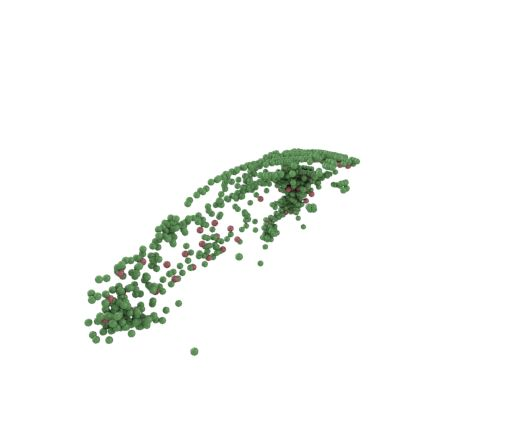
\includegraphics[width=1.75cm,trim={\cropleft cm \croplower cm \cropright cm \cropupper cm},clip]{gdat_kitti_2448_gt}
        \end{subfigure}
        \subcaption{KITTI, Point Clouds}
    \end{subfigure}
    \begin{subfigure}[t]{0.235\textwidth}
        \vspace{0px}\centering
        \begin{subfigure}[t]{0.48\textwidth}
            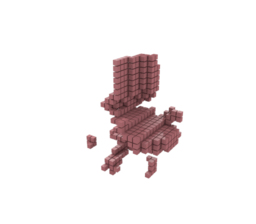
\includegraphics[width=1.75cm,trim={\cropleft cm \croplower cm \cropright cm \cropupper cm},clip]{gdat_yang_chair_1_bin_points}
        \end{subfigure}
        \begin{subfigure}[t]{0.48\textwidth}
            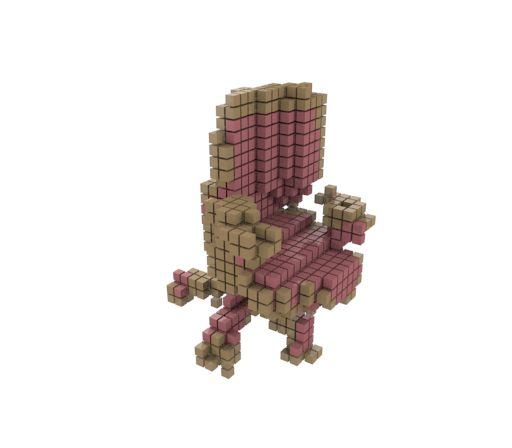
\includegraphics[width=1.75cm,trim={\cropleft cm \croplower cm \cropright cm \cropupper cm},clip]{gdat_yang_chair_1_bin}
        \end{subfigure}
        \\
        \begin{subfigure}[t]{0.48\textwidth}
            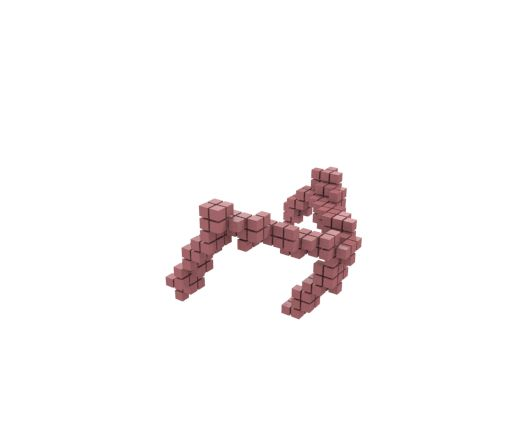
\includegraphics[width=1.75cm,trim={\cropleft cm \croplower cm \cropright cm \cropupper cm},clip]{gdat_yang_table_5_bin_points}
        \end{subfigure}
        \begin{subfigure}[t]{0.48\textwidth}
            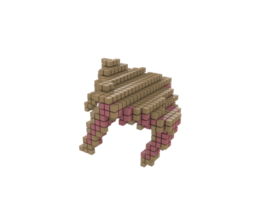
\includegraphics[width=1.75cm,trim={\cropleft cm \croplower cm \cropright cm \cropupper cm},clip]{gdat_yang_table_5_bin}
        \end{subfigure}
        \subcaption{\Kinect, Occupancy Grids}
    \end{subfigure}
    \vspace*{-\figskipcaption px}
	\caption{{{\bf Extracted KITTI and \Kinect Data.} For KITTI, we show observed points in {\color{rred}red} and the accumulated, partial ground truth in {\color{rgreen}green}. Note that for the first example ground truth is not available due to missing past/future observations. For \Kinect, we show observations in {\color{rred}red} and ElasticFusion \citep{Whelan2015RSS} ground truth in {\color{rbeige}beige}. Note that the objects are rotated and not aligned as in ModelNet (\cf \figref{fig:data-shapenet-modelnet}).}}
	\label{fig:data-kitti-yang}
    \vspace*{-\figskipbelow px}
\end{figure}